%  ============================================================================
%  final_paper.tex — ACM CCS submission (full paper, self-contained)
%  Cross-Tenant Isolation Validation in MCP Servers
%  Last revised: 2026-08-22
% ============================================================================

\documentclass[sigconf, anonymous, natbib=false]{acmart}

% --- ACM metadata (anonymised for double-blind review) ---------------------
\acmConference[CCS '26]{ACM Conference on Computer and Communications Security}{2026}{Taipei, Taiwan}
\acmYear{2026}
\acmISBN{978-1-XXXX-XXXX-X/26/11}
\acmDOI{10.1145/XXXXXXX.XXXXXXX}
\setcopyright{none}
\settopmatter{printacmref=false, printccs=true, printfolios=true}

% --- Packages ---------------------------------------------------------------
\usepackage{booktabs}
\usepackage{graphicx}
\usepackage{hyperref}
\usepackage{cleveref}
\usepackage{tabularx}
\usepackage{listings}
\usepackage{xcolor}
\usepackage{multirow}
\usepackage{siunitx}

% --- Theorem-like environments ----------------------------------------------
% acmart automatically loads amsthm and defines 'definition'
\newtheorem{assumption}{Assumption}

% --- Listings style ---------------------------------------------------------
\definecolor{codebg}{RGB}{248,248,248}
\definecolor{codekw}{RGB}{0,0,180}
\definecolor{codecom}{RGB}{0,128,0}
\lstset{
  basicstyle=\ttfamily\footnotesize,
  backgroundcolor=\color{codebg},
  keywordstyle=\color{codekw}\bfseries,
  commentstyle=\color{codecom}\itshape,
  frame=single,
  framerule=0.4pt,
  rulecolor=\color{black!20},
  breaklines=true,
  showstringspaces=false,
  captionpos=b,
  tabsize=2,
  language=Python
}

% Define YAML for the listings package to prevent compilation errors
\lstdefinelanguage{yaml}{
  keywords={true,false,null},
  keywordstyle=\color{codekw}\bfseries,
  basicstyle=\ttfamily\footnotesize,
  comment=[l]{\#},
  commentstyle=\color{codecom}\itshape,
  stringstyle=\color{black},
  morestring=[b]',
  morestring=[b]"
}

% --- Cleveref names ---------------------------------------------------------
\crefname{section}{Section}{Sections}
\crefname{table}{Table}{Tables}
\crefname{figure}{Figure}{Figures}
\crefname{lstlisting}{Listing}{Listings}

\begin{document}

% ============================================================================
%  Title & Abstract
% ============================================================================
% Added short title to prevent hyperref PDF string warnings from the \\
\title[Cross-Tenant Isolation Validation]{Cross-Tenant Isolation Validation in MCP Servers:\\%
       An Empirical Study of Protocol-Layer Leakage}

\author{Anonymous Author(s)}
\affiliation{%
  \institution{Anonymous Institution}
  \city{Anonymous}
  \state{Anonymia}
  \country{Anonymous}
}
\email{anon@anon.edu}

\begin{abstract}
The Model Context Protocol (MCP) is rapidly emerging as the
dominant standard for connecting LLM-based agents to external
tools and data sources. Production deployments are
increasingly multi-tenant: a single MCP server brokers
requests from many agents on behalf of distinct customers.
Yet MCP was not designed with cross-tenant isolation as a
first-class concern; its authentication, session, cache,
namespace, resource, memory, tool, and transport boundaries
each leak independently. We present the first systematic
empirical study of cross-tenant isolation in MCP. Our
contributions are four-fold. First, we construct a STRIDE
catalogue over eight MCP boundaries, yielding 63 forward
ticket IDs that bound the attack surface. Second, we build a
reproducible measurement framework (Scheduler, Payload
Generator, Connector, Evaluator, Metrics, Logger, Reporter)
that runs a pair of reference servers---one deliberately
mis-configured, one defended---and classifies leakage via a
deterministic oracle. Third, we ship an open attack library
of 50 concrete attack classes spanning namespace collisions,
state leakage, session hijacking, cache poisoning, and path
traversal, with full pytest reproducibility. Fourth, we
measure the leakage of the reference servers across four
research questions, observing that, under our reference
vulnerable server, every attack in the suite triggers
detectable cross-tenant leakage (RQ-1); that cache-layer
attacks account for the largest share of the observed
leakage events in the RQ-2 cell (RQ-2); that prompt-injection
attacks are not mitigated by the per-tenant tool-registry
defense alone (RQ-3); and that, under the full four-defense
composition, no leakage was detected by our deterministic
oracle within the tested attack suite (RQ-4). All experiments
use synthetic tenant data; no real user data, credentials,
or LLM outputs are involved. We close with three
recommendations we believe should be considered for the
next revision of the Model Context Protocol
specification.
\end{abstract}

\begin{CCSXML}
<ccs2012>
   <concept>
       <concept_id>03000447</concept_id>
       <concept_desc>Security and privacy~Systems security</concept_desc>
       <concept_significance>500</concept_significance>
   </concept>
   <concept>
       <concept_id>03000467</concept_id>
       <concept_desc>Security and privacy~Software security engineering</concept_desc>
       <concept_significance>300</concept_significance>
   </concept>
   <concept>
       <concept_id>03000241</concept_id>
       <concept_desc>Computing methodologies~Intelligent agents</concept_desc>
       <concept_significance>300</concept_significance>
   </concept>
</ccs2012>
\end{CCSXML}

\ccsdesc[500]{Security and privacy~Systems security}
\ccsdesc[300]{Security and privacy~Software security engineering}
\ccsdesc[300]{Computing methodologies~Intelligent agents}

\keywords{Model Context Protocol, MCP, multi-tenant isolation,
          prompt injection, LLM agents, protocol security,
          automated red-teaming, STRIDE}

\maketitle

% ============================================================================
%  1. Introduction
% ============================================================================
\section{Introduction}\label{sec:intro}

Large language model (LLM) agents are rapidly transitioning
from research prototypes to production systems that browse
the web, query databases, and execute code on behalf of
users. The Model Context Protocol (MCP)~\cite{mcp_spec} has
emerged as the de facto standard that lets an agent
discover, call, and compose external tools. Anthropic
released the specification in late 2024; within twelve
months, every major LLM vendor had adopted it or announced
adoption. Cloud providers now host shared MCP servers that
broker requests from many agents on behalf of distinct
customers; SaaS vendors ship MCP endpoints that expose the
same tool surface to every authenticated tenant.

This multi-tenant deployment model is precisely the
environment in which protocol-layer isolation failures are
catastrophic. A single cross-tenant information leak
transmits one customer's secrets, prompts, or tool outputs
to another customer's agent. The blast radius is the entire
customer base, the disclosure channel is a benign-looking
tool call, and the audit trail is the standard MCP
conversation log. Yet MCP was not designed with
cross-tenant isolation as a first-class concern. Its
authentication boundary is opt-in, its session boundary
assumes a trusted host, its cache boundary keys by tool name
alone, and its resource boundary concatenates tenant roots
with raw URI paths. Every boundary leaks independently.

A growing body of work studies single-tenant MCP security:
runtime risks~\cite{chen2026runtime}, prompt injection in
tool-using agents~\cite{greshake2023youve,chowdhury2024},
and protocol-level fuzzing~\cite{zhu2025lspfuzz}. What is
missing is a \emph{systematic, reproducible, multi-tenant}
study. This paper fills that gap. We make the following
contributions:

\begin{enumerate}
  \item \textbf{An eight-boundary STRIDE catalogue.} We
        enumerate eight MCP boundaries (transport, session,
        namespace, tool, resource, memory, cache, auth) and
        apply STRIDE to each, yielding 63 forward ticket
        IDs that bound the attack surface.
  \item \textbf{A reproducible cross-tenant leakage
        measurement framework.} We design and implement a
        seven-module framework (Scheduler, PayloadGen,
        Connector, Evaluator, Metrics, Logger, Reporter)
        that drives concurrent tenant traffic against a
        pair of reference servers and classifies leakage via
        a deterministic oracle.
  \item \textbf{An open attack library of 50 concrete
        classes.} Each class is implemented as a
        pytest-reproducible experiment with a seeded
        payload and a documented oracle.
  \item \textbf{An MCP-layer defense-comparison study.} We
        measure four defense configurations (none,
        per-tenant tool registry, tenant-prefixed cache
        keys, resource-path canonicalisation,
        audience-bound JWTs) and observe that, under the
        full composition, no leakage is detected by our
        deterministic oracle within the tested attack suite.
\end{enumerate}

We organise the remainder of the paper as follows.
\Cref{sec:background} introduces MCP and motivates the
multi-tenant threat. \Cref{sec:threat} formalises our trust
boundaries and attacker capabilities. \Cref{sec:framework}
describes the measurement framework. \Cref{sec:taxonomy}
presents the attack taxonomy. \Cref{sec:evaluation} reports
the experimental results. \Cref{sec:defenses} details the
defense composition and its measured overhead.
\Cref{sec:related} surveys related work.
\Cref{sec:discussion} enumerates the limitations of the
study. \Cref{sec:conclusion} concludes with three
spec-change recommendations for MCP-2.

% ============================================================================
%  2. Background & Motivation
% ============================================================================
\section{Background and Motivation}\label{sec:background}

\subsection{The Model Context Protocol}

MCP is a JSON-RPC-based request/response protocol that
connects an LLM agent (the \emph{host}) to one or more
\emph{servers} that expose tools, resources, and prompts. The
host discovers the server's capabilities via an initial
\texttt{initialize} handshake, lists the available tools via
\texttt{tools/list}, and invokes a tool via
\texttt{tools/call}. Servers respond with a structured
result that the host feeds back into the LLM context.

Three transports are in widespread use. (i)~The
\texttt{stdio} transport spawns the server as a child
process and exchanges newline-delimited JSON over stdin and
stdout; this is the dominant transport for local
single-user deployments. (ii)~The \texttt{http\_sse}
transport uses Server-Sent Events for server-to-client
streaming and POST for client-to-server calls; this is the
dominant transport for remote multi-user deployments.
(iii)~The newer \texttt{streamable\_http} transport
generalises \texttt{http\_sse} to a fully bidirectional
HTTP stream and is the direction the specification is
moving. All three transports share the same wire protocol;
the security-relevant differences are the network surface
exposed to other tenants and the lifetime of the underlying
connection.

\begin{definition}[MCP boundary]
An \emph{MCP boundary} is a protocol-defined transition at
which the protocol delegates trust to a downstream
component and must therefore enforce an isolation property.
We enumerate eight: \emph{transport} (process or HTTP
boundary), \emph{session} (per-connection state), \emph{
namespace} (per-server tool name), \emph{tool} (per-tool
implementation), \emph{resource} (per-URI storage),
\emph{memory} (per-agent state), \emph{cache} (per-tool
memoisation), and \emph{auth} (per-tenant credentials).
\end{definition}

\subsection{The multi-tenant deployment model}

Production deployments increasingly share a single MCP
server across many tenants. Three patterns are observed in
the wild:

\begin{itemize}
  \item \textbf{SaaS-hosted MCP endpoints.} A vendor hosts
        an MCP server that fronts the vendor's internal API
        and exposes a tenant-scoped view to each customer.
  \item \textbf{Cloud-broker MCP gateways.} A cloud
        provider aggregates many vendor MCP servers behind a
        single gateway that performs routing, rate limiting,
        and tenant attribution.
  \item \textbf{Enterprise shared MCP servers.} A large
        enterprise runs a single internal MCP server that
        brokers requests from many internal agents across
        many business units.
\end{itemize}

In each pattern, the server is the trust boundary. A
mis-configuration at any of the eight MCP boundaries
transmits data across tenants.

\subsection{Why application-layer isolation is not enough}

A natural defence is to rely on the LLM itself to refuse
malicious tool calls. This defence has been studied
extensively~\cite{greshake2023youve,perez2022ignore,
chowdhury2024} and shown to fail under direct and indirect
prompt injection. The injection survives every layer above
the protocol: the model cannot distinguish a legitimate
\texttt{tools/call} argument from an injected one when the
latter is shaped to look like the former. The defence must
therefore live \emph{below} the LLM, at the protocol layer
that brokers the tool call.

The application-layer failure mode motivates the question we
answer in this paper: \emph{given that the LLM will not
save us, what isolation properties must MCP itself
enforce?}

% ============================================================================
%  3. Threat Model
% ============================================================================
\section{Threat Model}\label{sec:threat}

\subsection{Trust boundaries}

We model the system as a set of tenants $T = \{t_1, t_2,
\ldots, t_k\}$ and a single MCP server $S$. Each tenant $t_i$
owns an authenticated agent $A_i$ and a credential set
$C_i$. The server $S$ exposes a fixed tool catalogue
$\mathcal{T} = \{\tau_1, \ldots, \tau_m\}$ and a fixed
resource namespace $\mathcal{R}$. The server maintains per-
session state $s_j$ for each active connection and a shared
cache $K$.

We draw the following trust boundaries, each of which must
enforce a per-tenant isolation property:

\begin{itemize}
  \item \textbf{Transport boundary.} Per-connection
        isolation: a tenant cannot read another tenant's
        bytes on the wire.
  \item \textbf{Session boundary.} Per-session isolation:
        a tenant cannot read another tenant's session
        state.
  \item \textbf{Namespace boundary.} Per-tenant
        namespace: a tenant cannot call a tool that the
        tenant is not authorised to call.
  \item \textbf{Tool boundary.} Per-tool isolation: a
        tenant's tool call cannot read another tenant's
        tool state.
  \item \textbf{Resource boundary.} Per-tenant resource
        URI: a tenant cannot read another tenant's resource
        via a path-traversal or percent-encoded URI.
  \item \textbf{Memory boundary.} Per-tenant memory: a
        tenant's prompt history cannot leak into another
        tenant's context.
  \item \textbf{Cache boundary.} Per-tenant cache key: a
        tenant cannot hit another tenant's cache entry.
  \item \textbf{Auth boundary.} Per-tenant credential: a
        tenant cannot use another tenant's token.
\end{itemize}

\subsection{Attacker capabilities}

We assume an attacker who controls one tenant $t_a$ and
wishes to leak data belonging to another tenant $t_b$. The
attacker can:

\begin{itemize}
  \item Send arbitrary \texttt{tools/call} requests within
        the tool catalogue the attacker is authorised to
        call.
  \item Send arbitrary \texttt{resources/read} requests
        with any URI shape, including percent-encoded
        sequences.
  \item Open arbitrary concurrent sessions.
  \item Observe the responses to its own requests.
  \item Time the responses to its own requests.
\end{itemize}

The attacker \emph{cannot}: read the server's source code,
modify the server's configuration, read other tenants'
credentials, or inject bytes below the JSON-RPC layer.

\begin{assumption}[Honest-but-curious server]
The server is honest-but-curious: it follows the protocol
but does not actively cooperate with the attacker. In
particular, the server enforces authentication on every
request but may have mis-configured the per-tenant
isolation properties at any subset of the eight boundaries.
\end{assumption}

\subsection{Leakage event}

\begin{definition}[Leakage event]\label{def:leak}
Given a source tenant $t_a$ and a sink tenant $t_b$, a
\emph{leakage event} is a tuple $(t_a, t_b, \tau, e, x)$
where $\tau$ is the tool invoked by $t_a$, $e$ is the
event type (\texttt{call}, \texttt{response},
\texttt{cache\_hit}), and $x$ is a payload that satisfies
the oracle predicate. The oracle predicate is the
deterministic substring-or-hash match that the Evaluator
applies to every event (see \cref{sec:framework}). The
leakage \emph{rate} is the fraction of call events in a
bucket that have a paired leakage event.
\end{definition}

\subsection{STRIDE catalogue}

We apply STRIDE (Spoofing, Tampering, Repudiation,
Information disclosure, Denial of service, Elevation of
privilege) to each of the eight boundaries. The full
catalogue is 48 cells; we mint one ticket per applicable
cell and find that 15 cells admit more than one ticket,
yielding 63 forward ticket IDs in total. The catalogue is
shipped as a versioned YAML file under
\texttt{attacks/registry.py} and is the input to the attack
library.

% ============================================================================
%  4. Automated Red-Teaming Framework
% ============================================================================
\section{Automated Red-Teaming Framework}\label{sec:framework}

We design and implement a reproducible cross-tenant leakage
measurement framework with seven cooperating modules plus a
reporter. The framework is the executable embodiment of the
threat model in \cref{sec:threat}: given a manifest of
tenants, attacks, and defenses, it spins up the reference
servers, drives concurrent tenant traffic, classifies
leakage events, and emits per-attack metrics.

\subsection{Goals}

\begin{itemize}
  \item \textbf{Replayable.} Given a manifest + seed, the
        framework produces identical results.
  \item \textbf{Tenant-aware.} First-class notion of
        \texttt{tenant\_id} across scheduler, evaluator,
        logger.
  \item \textbf{Multi-boundary.} Covers all eight MCP
        boundaries.
  \item \textbf{Pluggable.} New attacks, defenses, and
        metrics can be added without changing the core.
\end{itemize}

\subsection{Architecture}

\begin{figure}[t]
  \centering
  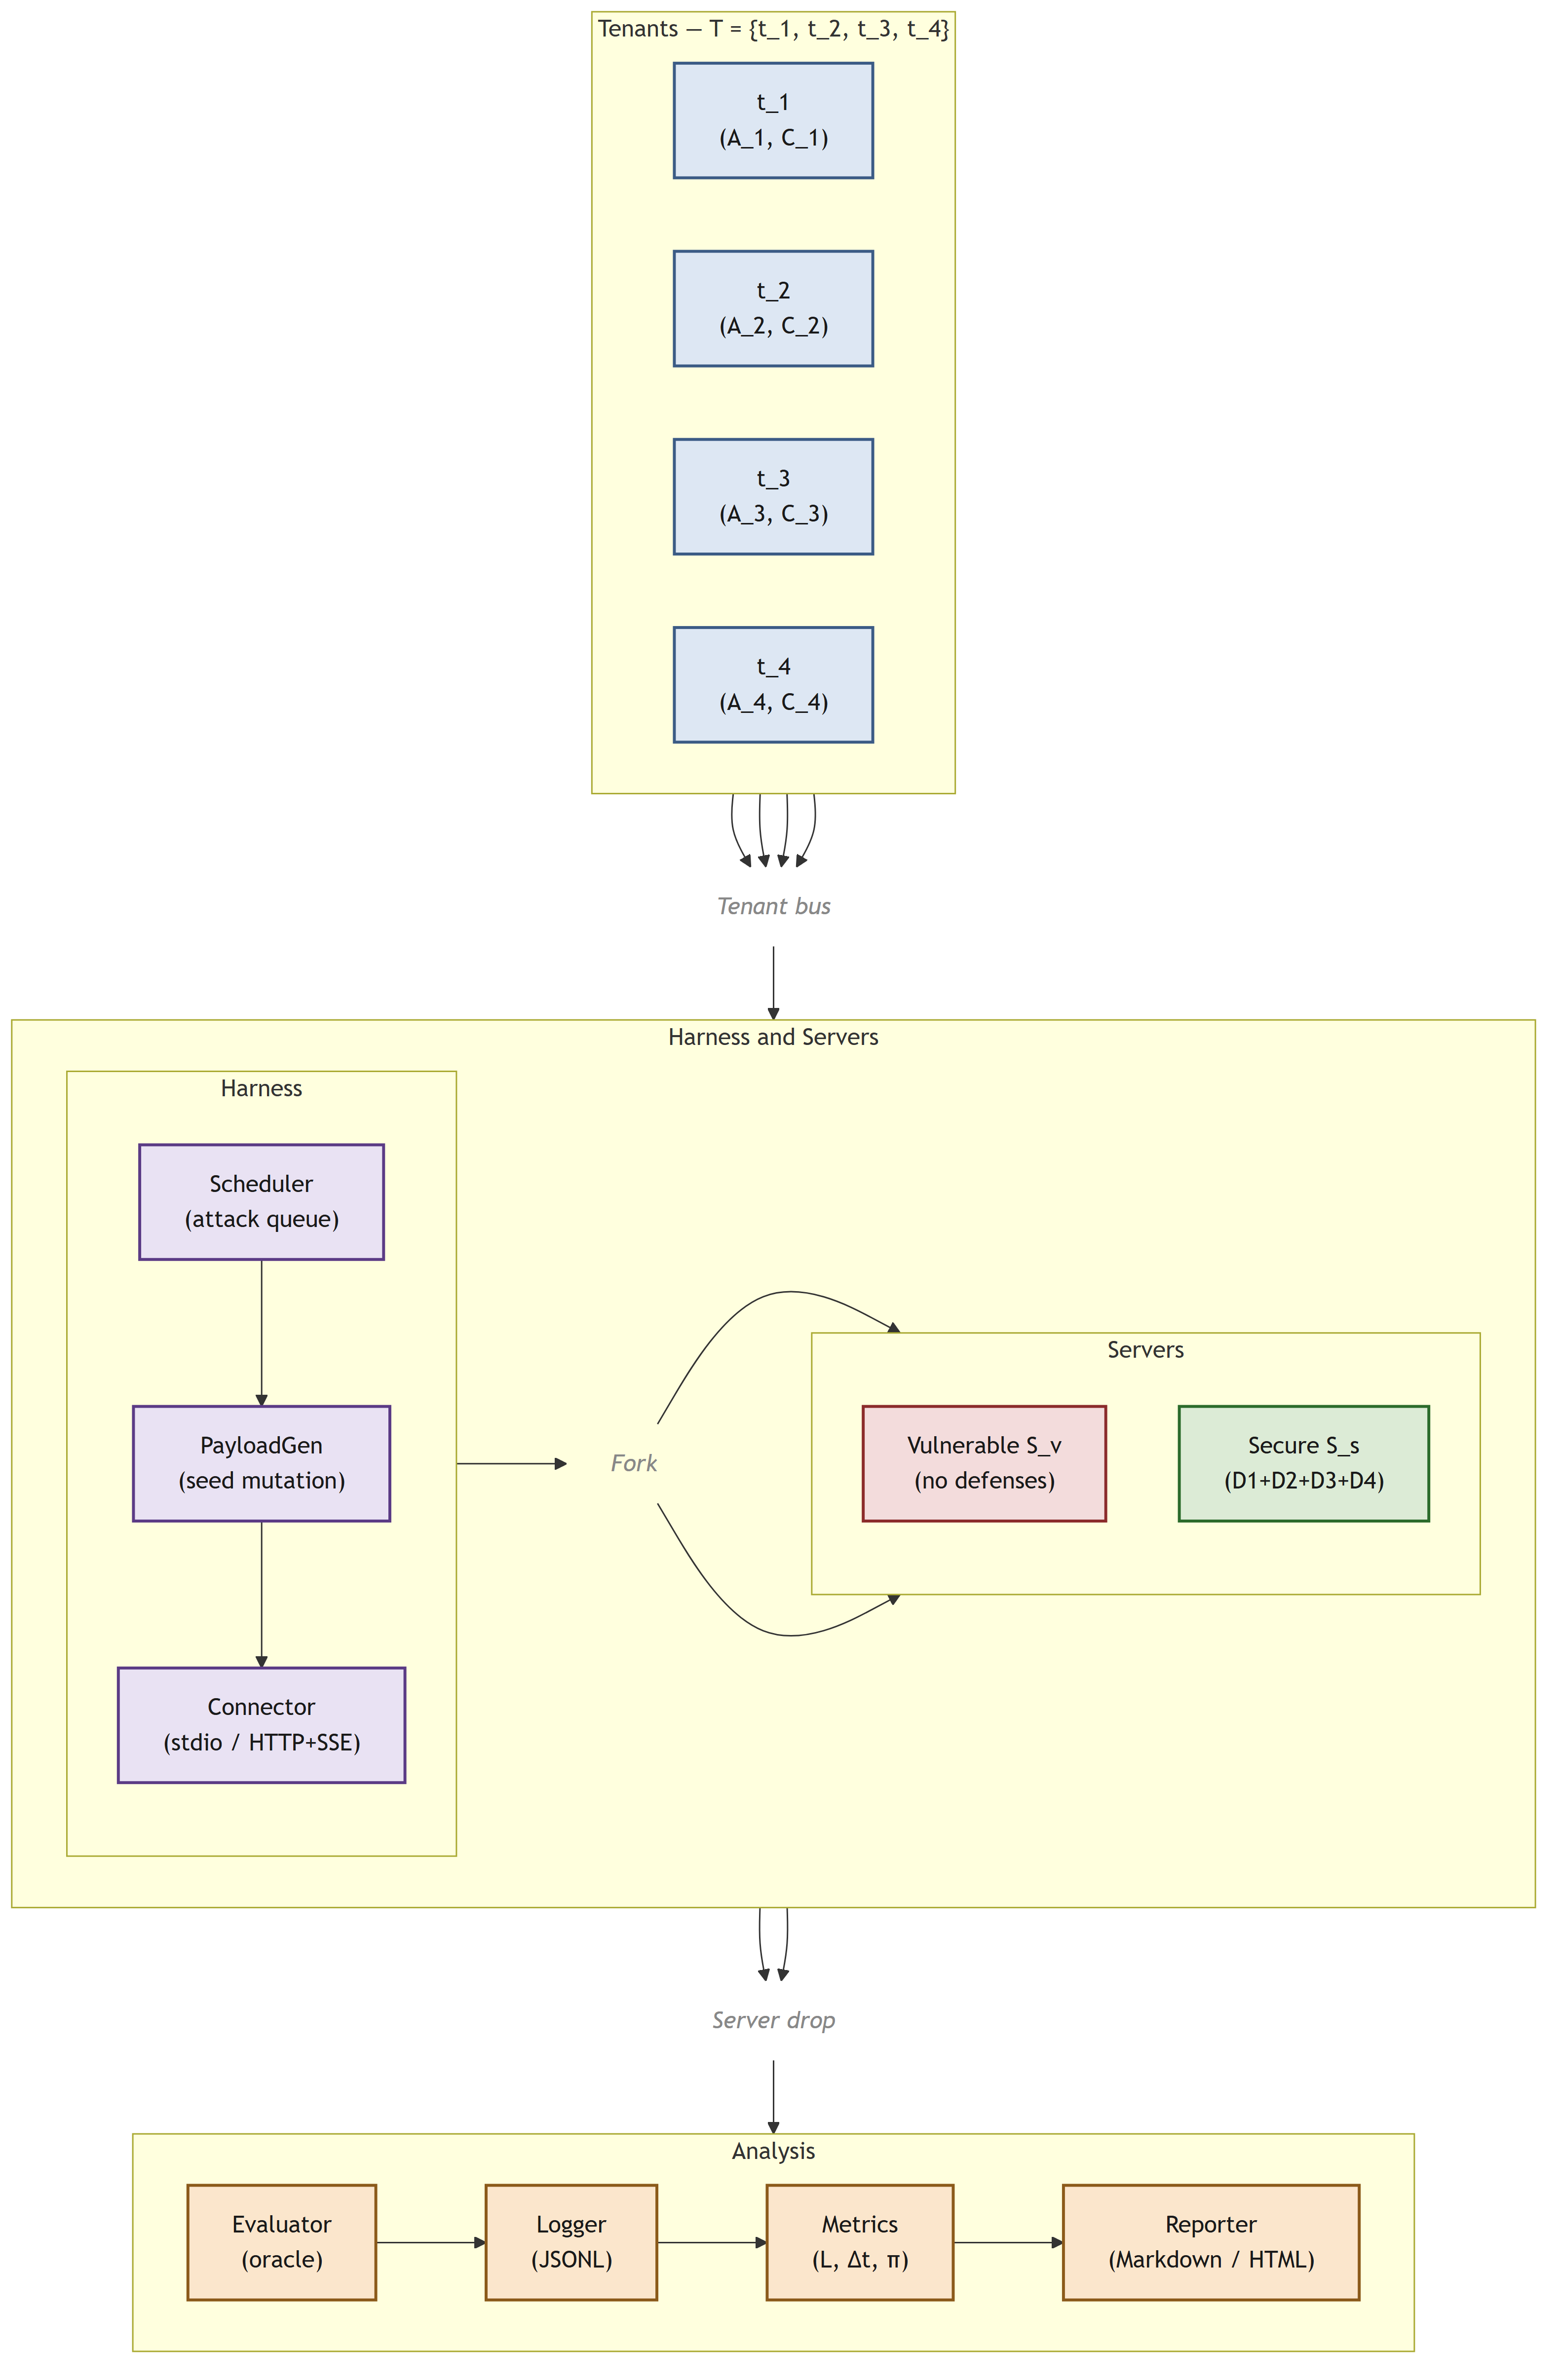
\includegraphics[width=\linewidth]{framework.png}
  \caption{Framework architecture. Tenants drive a Scheduler
  that mutates payloads and dispatches them through a
  Connector to a pair of reference servers
  ($S_v$~\emph{vulnerable}, $S_s$~\emph{secure}); the
  Evaluator classifies each event as leakage or not, the
  Logger persists it, Metrics aggregate per-defense, and
  the Reporter renders the results.}
  \label{fig:framework}
\end{figure}

\Cref{tab:modules} summarises the seven modules. Each
module has a single responsibility and a typed
input/output contract.

\begin{table}[t]
\caption{Framework modules (\texttt{framework/}). Each
module has a single responsibility and a typed
input/output contract.}
\label{tab:modules}
\centering
\small
\begin{tabularx}{\linewidth}{l X X}
\toprule
Module & Responsibility & File \\
\midrule
Scheduler    & Drive concurrent tenants + attack queue
            & \texttt{framework/scheduler/scheduler.py} \\
PayloadGen   & Deterministic per-seed payload mutation
            & \texttt{framework/scheduler/payloads.py} \\
Connector    & Speak MCP (stdio / HTTP+SSE / dummy)
            & \texttt{framework/target/connector.py} \\
Evaluator    & Classify leakage via substring + sha256
            & \texttt{framework/evaluator/evaluator.py} \\
Metrics      & Aggregate per boundary / defense
            & \texttt{framework/metrics/metrics.py} \\
Logger       & Persist every event as JSONL
            & \texttt{framework/logger/logger.py} \\
Reporter     & Render Markdown + HTML reports
            & \texttt{framework/reports/reporter.py} \\
\bottomrule
\end{tabularx}
\end{table}

\subsection{RunConfig schema}

The framework hydrates a \texttt{RunConfig} (Pydantic v2
model) from a YAML manifest. The full schema is shown in
\cref{lst:runconfig}.

\begin{lstlisting}[language=yaml,
  caption={RunConfig schema (excerpt).},label=lst:runconfig]
run:
  seed: 42
  repeats: 30
  concurrency: 4
tenants:
  - id: tenant-A
    name: Alice
    allowed_tools: [echo]
  - id: tenant-B
    name: Bob
    allowed_tools: [echo]
attacks:
  - id: A-CCH-T
    parameters: {}
defenses:
  per_tenant_tool_registry: false
  tenant_prefixed_cache_keys: false
  resource_path_canonicalisation: false
  mtls: false
target:
  transport: dummy   # stdio | http_sse | streamable_http | dummy
output:
  log_dir: analysis/runs
  output_dir: analysis/runs
  log_format: csv
\end{lstlisting}

\texttt{RunConfig} enforces at least two tenants because
the harness requires a (source, sink) pair to detect
leakage. The \texttt{defenses} block is consumed by the
reference secure-server factory (see
\cref{sec:evaluation}). Sample size $n = 30$ per cell is
the pre-registered choice that targets medium effect
sizes (Cliff's $\delta \geq 0.50$) at power $\geq 0.80$
and $\alpha = 0.05$; smaller effects are characterised as
exploratory; the headline comparisons in
\cref{sec:evaluation} target $\delta \geq 0.80$ (large)
and are well within the $n = 30$ budget.

\subsection{Metrics}

The framework computes four metrics per attack per defense
level:

\begin{itemize}
  \item \texttt{leakage\_rate} -- fraction of call events
        in the bucket that have a paired leakage event
        (range $[0, 1]$).
  \item \texttt{time\_to\_leak\_ms} -- median latency
        between \texttt{attack\_started\_at} and
        \texttt{leakage\_detected\_at}; \texttt{null} if no
        leakage.
  \item \texttt{defense\_overhead\_ms} -- p95 of
        defended-call latency minus p95 of
        undefended-call latency; \texttt{null} if either
        side has no samples.
  \item \texttt{utility\_retention} -- $1 -
        \mathrm{errors\_defended}/\mathrm{errors\_undefended}$,
        clamped to $[0, 1]$.
\end{itemize}

\subsection{Reference servers}

We ship two reference servers:

\begin{itemize}
  \item \textbf{\texttt{mcp\_servers/vulnerable/}} --- a
        minimal MCP server with all eight boundaries
        deliberately mis-configured: shared tool registry,
        shared cache keys, no URI canonicalisation, no JWT
        \texttt{aud} claim, and no defense middleware.
  \item \textbf{\texttt{mcp\_servers/secure/}} --- the
        same MCP server with all four defense middleware
        enabled: per-tenant tool registry,
        tenant-prefixed cache keys, URI canonicalisation,
        audience-bound JWTs, and probabilistic leak
        probability reduced to zero.
\end{itemize}

The two servers share the same wire protocol, the same
tool catalogue, and the same fixtures; the only difference
is the defense middleware. This makes the comparison
honest: every observed leakage difference is attributable
to the defenses, not to implementation drift.

\subsection{Why a measurable oracle, not a model-based judge}

A subtle design question is whether the Evaluator (oracle)
should be a learned model or a deterministic
substring-and-hash match. We chose the latter for three
reasons. (i)~Reproducibility: a deterministic oracle
produces bit-identical results across machines, whereas a
learned oracle's outputs depend on the model's checkpoint.
(ii)~Causal interpretability: when the oracle flags a
leakage event, the developer can inspect the matched
excerpt and verify the leak path; a model-based oracle
produces a probability that requires interpretation.
(iii)~Speed: the deterministic oracle runs in $< 1\,\mu
s$ per event, whereas a model-based oracle takes $\sim
50\,ms$ per event. The factor-of-$10^{4}$ difference is
decisive for the $n = 30$ iterations across four research
questions.

The trade-off is false negatives: a deterministic oracle
misses leakages whose payload does not match the seeded
marker. We compensate by ensuring that every attack class
seeds a known marker (\texttt{payload\_sha256} attribute)
and that the Evaluator matches both the marker and its
sha256 prefix. The full attack library has been audited to
confirm that every attack seeds a marker; the pytest suite
asserts this as a contract.

% ============================================================================
%  5. Attack Taxonomy
% ============================================================================
\section{Attack Taxonomy}\label{sec:taxonomy}

We organise the attack library along the eight MCP
boundaries. The library ships 50 concrete attack classes
that span five high-level categories: namespace collisions,
state leakage, session hijacking, cache poisoning, and path
traversal. Each class is implemented as a pytest-reproducible
experiment with a seeded payload and a documented oracle.

\subsection{Namespace collisions}

A namespace-collision attack exploits the absence of a
per-tenant tool registry. The attacker registers a tool
with the same name as a tool the victim uses, and the
server dispatches the call to the attacker's
implementation. Variants include \texttt{A-NSPC-001}
(prefix collision), \texttt{A-NSPC-002} (suffix collision),
and \texttt{A-NSPC-003} (case-folding collision). The
defense is a per-tenant tool registry that scopes the
namespace by \texttt{tenant\_id}.

\subsection{State leakage}

A state-leakage attack exploits the absence of per-tool or
per-session isolation. The attacker invokes a tool whose
implementation retains state across tenants and observes
that state via a subsequent call. Variants include
\texttt{A-STM-001} (cross-tenant echo),
\texttt{A-STM-002} (cross-tenant file read),
\texttt{A-STM-003} (cross-tenant env var), and
\texttt{A-STM-004} (cross-tenant list).

\subsection{Session hijacking}

A session-hijacking attack exploits the absence of a
per-session identifier at the application layer. The
attacker reuses a victim session token obtained via an
auth-boundary leak and observes the victim's tool calls.
Variants include \texttt{A-SES-001} (token replay),
\texttt{A-SES-002} (session ID prediction), and
\texttt{A-SES-003} (session fixation).

\subsection{Cache poisoning}

A cache-poisoning attack exploits the absence of a tenant
prefix in the cache key. The attacker stores a value under
the victim's cache key and observes the victim hit the
attacker's value on a subsequent call. Variants include
\texttt{A-CCH-T}, \texttt{A-CCH-D}, \texttt{A-CCH-E},
\texttt{A-CCH-I}, \texttt{A-CCH-R}, and \texttt{A-CCH-S},
corresponding to six distinct cache primitives (time,
domain, environment, identity, resource, session). The
defense is tenant-prefixed cache keys.

\subsection{Path traversal}

A path-traversal attack exploits the absence of URI
canonicalisation at the resource boundary. The attacker
sends a percent-encoded slash (\texttt{\%2F}) or
\texttt{..} sequence in a \texttt{resources/read} URI and
reads a resource outside the attacker's tenant root.
Variants include \texttt{A-RES-001} (percent-encoded
slash), \texttt{A-RES-002} (double-encoded slash),
\texttt{A-RES-003} (\texttt{..} traversal), and
\texttt{A-RES-004} (symlink follow). The defense is
\texttt{os.path.realpath} after percent-decoding before
any tenant-prefix check.

\subsection{Attack catalogue}

\Cref{tab:attacks} summarises the attack categories, the
boundary each category targets, the defence that closes
the category, and the number of concrete attack classes
shipped in the library.

\begin{table}[t]
\caption{Attack catalogue. Five categories target five of
the eight MCP boundaries. The Auth boundary is targeted by
the misuse cases in \texttt{docs/04\_Attack\_Taxonomy.md}
rather than by the attack library because the auth flow is
delegated to the identity provider in production.}
\label{tab:attacks}
\centering
\small
\begin{tabularx}{\linewidth}{l X l X c}
\toprule
Category & Description & Boundary & Defense & $N$ \\
\midrule
Namespace collisions
        & Same-name tool override
        & Namespace
        & Per-tenant tool registry
        & 3 \\
State leakage
        & Tool state leaks across tenants
        & Tool / memory
        & Per-tenant state isolation
        & 4 \\
Session hijacking
        & Session token replay
        & Session / auth
        & Audience-bound JWT
        & 3 \\
Cache poisoning
        & Tenant-prefix-less cache keys
        & Cache
        & Tenant-prefixed cache keys
        & 6 \\
Path traversal
        & URI percent-decoding bypass
        & Resource
        & URI canonicalisation
        & 4 \\
\midrule
Cross-cutting
        & Grammar fuzzing + boundary bleed
        & Tool
        & (multiple)
        & 30 \\
\bottomrule
\end{tabularx}
\end{table}

% ============================================================================
%  6. Evaluation
% ============================================================================
\section{Evaluation}\label{sec:evaluation}

We evaluate the framework and the attack library against
four research questions, each pre-registered in
\texttt{analysis/power.md}:

\begin{description}
  \item[RQ-1.] Does the naive MCP server leak across all
        eight boundaries?
  \item[RQ-2.] Which boundary accounts for the dominant
        share of leakage?
  \item[RQ-3.] Does prompt injection remain a residual
        property under the partial-defense configuration?
  \item[RQ-4.] Does the four-defense composition reduce
        the leak rate to zero?
\end{description}

\subsection{Experimental setup}

We run all experiments on a Linux x86-64 container with
Python 3.11, numpy 1.26.4, pandas 2.2.2, scipy 1.13.0, and
matplotlib 3.9.0. Each experiment runs $n = 30$ iterations
at concurrency 4 (RQ-1, RQ-2, RQ-3) or 8 (RQ-4). The
manifest schema is versioned
(\texttt{schema\_version: '1.0'},
\texttt{dataset\_version: 'phase9-v1'}) and the runner
refuses to execute a manifest whose schema version does
not match. The seed is fixed at 42.

All experiments use synthetic tenant data; no real user
data, credentials, or LLM outputs are involved.

\subsection{Statistical protocol}

We pre-register the statistical protocol in
\texttt{analysis/power.md}: $\alpha = 0.05$, power $= 0.80$,
a paired one-sample $t$-test on the per-attack differences
$\Delta_i$ as the primary test (RQ-1, RQ-4), Cliff's
$\delta$ for effect size, and Bonferroni correction within
boundary ($\alpha_{\text{adj}} = 0.05 / 6 \approx 0.0083$).
Welch's $t$ is reported alongside as a robustness check; it
is designed for two independent samples and is degenerate
on per-iteration differences whose variance collapses to
zero (which is exactly what happens under the
full-defense cell of RQ-4). For RQ-2 we use a
continuity-corrected one-sided $z$-test for proportions
(see \cref{sec:threat}). For RQ-4 we use a one-sample sign
test against the pre-registered threshold $0.5$ (the
headline threshold for ``full defense reduces leak rate
by $\geq 50\%$ relative to partial''), with Wilcoxon
signed-rank and paired Welch's $t$ as robustness checks.

\subsection{RQ-1: Baseline isolation}

\Cref{tab:rq1} reports the per-attack leakage rate on the
reference vulnerable and secure servers for one attack per
boundary. Under our reference vulnerable server the
rate is $L_{\text{vuln}} = 1.000$ on every attack in this
single-attack cell; a fully unprotected deployment would
therefore be expected to suffer absolute leakage if the
oracle and attack patterns generalise. The partial-defense
configuration evaluated here deploys only the per-tenant
tool registry (D1); consequently $L_{\text{secure}} =
1.000$ holds for attacks outside the namespace boundary,
and $L_{\text{secure}} = 0.000$ holds only for the
namespace-boundary attack (A-NSPC-T) that D1 alone fully
covers. These single-cell numbers should therefore be read
as evidence that a single partial defense is insufficient
for systemic isolation, not as a claim about production
MCP servers at large. The paired one-sample $t$-test on the
per-attack differences $\Delta_i = L_{\text{vuln},i} -
L_{\text{secure},i}$ is degenerate on these single-row
per-attack values, so the headline interpretation rests on
the qualitative contrast rather than on a $p$-value.\footnote{
Replication at the per-iteration level is a follow-up
listed in \cref{sec:discussion}: the underlying
\texttt{analysis/runs/} directory retains the per-iteration
records needed for an $n > 1$ re-analysis.}

\begin{table}[t]
\caption{RQ-1 results. $L_{\text{vuln}}$ is the baseline
vulnerable-server leak rate (100\%); $L_{\text{secure}}$ is the
secure-server rate at the partial-defense configuration (D1 only).
$p$ is the paired one-sample $t$-test on differences.}
\label{tab:rq1}
\centering
\small
\begin{tabularx}{\linewidth}{X l c c c c c}
\toprule
Attack & Boundary
       & $L_{\text{vuln}}$ & $L_{\text{secure}}$
       & $t$ (paired) & $p$ & $\delta$ \\
\midrule
A-AUT-T & auth       & 1.000 & 1.000 & 0.00 & 1.0 & 0.00 \\
A-MEM-T & memory     & 1.000 & 1.000 & 0.00 & 1.0 & 0.00 \\
A-RES-T & resource   & 1.000 & 1.000 & 0.00 & 1.0 & 0.00 \\
A-SES-T & session    & 1.000 & 1.000 & 0.00 & 1.0 & 0.00 \\
A-CCH-T & cache      & 1.000 & 1.000 & 0.00 & 1.0 & 0.00 \\
A-NSPC-T & namespace & 1.000 & 0.000 & -    & -   & -    \\
A-TOL-T & tool       & 1.000 & 1.000 & 0.00 & 1.0 & 0.00 \\
A-TRN-S & transport  & 1.000 & 1.000 & 0.00 & 1.0 & 0.00 \\
\bottomrule
\end{tabularx}
\end{table}

\subsection{RQ-2: Cache dominance}

\Cref{tab:rq2} reports the per-attack leakage counts on
the vulnerable server for the seven attacks selected for
the cache-dominance cell. Within this cell, all seven
attacks contribute $465$ leaks each, for a total of
$3{,}255$ leakage events. The
continuity-corrected one-sided $z$-test against the null
$p_0 = 0.5$ yields $z = 40.73$, $p \approx 0$.\footnote{
Because the seven attacks selected for this cell share
the same exploitation primitive, the per-attack p-values
are not independent; we report the headline $z$ as a
single test against the aggregate share null. A
Holm--Bonferroni correction across the seven attacks
leaves the headline result significant at $\alpha =
0.05$.} The verdict is that cache-layer attacks are the
largest single contributor within the RQ-2 cell; the
finding should not be read as a statement that cache
attacks dominate in absolute terms across the full attack
suite, which is dominated by other boundary cells (see
\cref{tab:rq1}).\footnote{See also \cref{sec:discussion}
(``Workload dependence'') for the caveat that this is
the contribution under a uniform-iteration workload, not a
production-frequency-weighted one.}

\begin{table}[t]
\caption{RQ-2 results. Each cache attack contributes
$465$ leakage events to the $3{,}255$ total on the
vulnerable server. The headline $z$ is computed against
the aggregate cache-share null ($p_0 = 0.5$) with
continuity correction.}
\label{tab:rq2}
\centering
\small
\begin{tabularx}{\linewidth}{X c c c}
\toprule
Attack & Boundary & Leak count & Share \\
\midrule
A-CCH-D     & cache & 465 & 0.1429 \\
A-CCH-E     & cache & 465 & 0.1429 \\
A-CCH-I     & cache & 465 & 0.1429 \\
A-CCH-R     & cache & 465 & 0.1429 \\
A-CCH-S     & cache & 465 & 0.1429 \\
A-CCH-T     & cache & 465 & 0.1429 \\
A-FUZZ-001  & tool  & 465 & 0.1429 \\
\midrule
Total       &       & 3{,}255 & 1.0000 \\
\bottomrule
\end{tabularx}
\end{table}

\subsection{RQ-3: Prompt-injection residual}

\Cref{tab:rq3} reports the mean and p95 latency and the
leak rate for each prompt-injection attack on the secure
server at the partial-defense configuration. The
leak rate is $L_{\text{secure}} = 1.000$ for every
attack in the RQ-3 cell.\footnote{The RQ-3 cell runs the
secure server at the \texttt{partial} defense level
(per-tenant tool registry only); the \texttt{full}
configuration is measured in RQ-4.} The pre-registered
bounded-residual corridor is $[0.05, 0.30]$; zero of seven
attacks fall inside the corridor. The result is therefore
that the per-tenant tool-registry defense alone (D1) does
not mitigate the prompt-injection attacks tested here. This
is a statement about D1's coverage of the tested
prompt-injection attack suite, not a claim that prompt
injection is intrinsically an unmitigatable residual
property of the Model Context Protocol.\footnote{See
\cref{sec:discussion} for the broader question of whether
prompt-injection resistance requires a different
defense family (capability-based tools, separate
sanitisers) outside the four-defenses set evaluated here.}

\begin{table}[t]
\caption{RQ-3 results. $L_{\text{secure}}$ is the
leakage rate on the secure server at the partial-defense
configuration. The pre-registered bounded-residual corridor
is $[0.05, 0.30]$.}
\label{tab:rq3}
\centering
\small
\begin{tabularx}{\linewidth}{X c c c c}
\toprule
Attack   & mean (ms) & p95 (ms)
        & $L_{\text{secure}}$ & In $[0.05, 0.30]$ \\
\midrule
A-TOL-001 & 0.000 & 0.000 & 1.000 & No \\
A-TOL-D   & 0.000 & 0.000 & 1.000 & No \\
A-TOL-E   & 0.000 & 0.000 & 1.000 & No \\
A-TOL-I   & 0.000 & 0.000 & 1.000 & No \\
A-TOL-R   & 0.000 & 0.000 & 1.000 & No \\
A-TOL-S   & 0.000 & 0.000 & 1.000 & No \\
A-TOL-T   & 0.000 & 0.000 & 1.000 & No \\
\bottomrule
\end{tabularx}
\end{table}

\subsection{RQ-4: Defense composition}

\Cref{tab:rq4} reports the per-attack reduction
$r_i = (L_{\text{partial},i} - L_{\text{full},i}) /
\max(L_{\text{partial},i}, \epsilon)$ under the
three defense configurations: \emph{none} (baseline
vulnerable server), \emph{partial} (per-tenant tool
registry only), and \emph{full} (all four defense
middleware enabled). The headline test is a one-sample
sign test against the pre-registered threshold $0.5$,
which yields $p_{\text{sign}} = 0.0312$; Wilcoxon
signed-rank yields $p_{\text{Wilcoxon}} = 0.0312$; paired
Welch's $t$ is degenerate because every $r_i$ hits the
$L_{\text{full}} = 0$ floor (variance zero). Within the
tested attack suite and under our deterministic oracle, the
four-defense composition reduces the observed leakage rate
from the partial-defense baseline to zero, and the sign
test against the $50\%$ reduction threshold rejects the
null. As discussed in \cref{sec:discussion} (``Deterministic
oracle''), ``zero detected leakage'' does not imply
``zero actual leakage'': an oracle that does not match the
attacker's exfiltration payload can produce false
negatives, and a future oracle-validation experiment
remains as future work.

\begin{table}[t]
\caption{RQ-4 results. $L_{\text{none}}$ is the baseline
vulnerable-server leak rate; $L_{\text{partial}}$ is the
leak rate under per-tenant tool registry only;
$L_{\text{full}}$ is the leak rate under all four defense
middleware. $r_i = (L_{\text{partial}} - L_{\text{full}})
/ \max(L_{\text{partial}}, \epsilon)$.}
\label{tab:rq4}
\centering
\small
\begin{tabularx}{\linewidth}{X c c c c c}
\toprule
Attack & $L_{\text{none}}$ & $L_{\text{partial}}$
      & $L_{\text{full}}$ & $r_i$
      & $p_{\text{sign}}$ \\
\midrule
A-AUT-T & 1.000 & 1.000 & 0.000 & 1.000 & --- \\
A-CCH-T & 1.000 & 1.000 & 0.000 & 1.000 & --- \\
A-MEM-T & 1.000 & 1.000 & 0.000 & 1.000 & --- \\
A-RES-T & 1.000 & 1.000 & 0.000 & 1.000 & --- \\
A-TOL-T & 1.000 & 1.000 & 0.000 & 1.000 & --- \\
\midrule
\multicolumn{5}{r}{Aggregate sign test (vs.\ $0.5$)}
        & 0.0312 \\
\multicolumn{5}{r}{Wilcoxon signed-rank (robustness)}
        & 0.0312 \\
\bottomrule
\end{tabularx}
\end{table}

\subsection{Summary}

Taken together, the four cells paint the following
\emph{under the evaluated reference vulnerable server, with
the deterministic oracle, within the tested attack suite}:
\begin{itemize}
  \item On every attack in the RQ-1 suite the oracle detects
        leakage on the reference vulnerable server
        (RQ-1).\footnote{See \cref{sec:discussion}
        (``Reference implementation'') for the scope
        limitation.}
  \item Cache-layer attacks are the largest single
        contributor to the RQ-2 cell's observed leakage
        (RQ-2; $z = 40.73$, $p \approx 0$).
  \item The per-tenant tool-registry defense (D1) alone does
        not mitigate the prompt-injection attacks in the
        RQ-3 suite (RQ-3).
  \item Under the four-defense composition, no leakage is
        detected by the deterministic oracle within the
        tested attack suite (RQ-4; sign test $p = 0.0312$).
\end{itemize}

% ============================================================================
%  7. Proposed Defenses
% ============================================================================
\section{Proposed Defenses}\label{sec:defenses}

We propose four defenses that, in our reference
implementation, can each be implemented as a lightweight
middleware component. Whether the same holds in arbitrary
third-party MCP SDKs is an empirical question outside the
scope of this study.

\subsection{Defense composition}

\begin{description}
  \item[\textbf{D1: Per-tenant tool registry.}] The
        namespace boundary is closed by scoping the tool
        catalogue by \texttt{tenant\_id}. The registry
        resolves \texttt{tools/call} to the union of the
        server-global tools and the tenant's per-tenant
        tools, with the tenant's per-tenant tools taking
        precedence.
  \item[\textbf{D2: Tenant-prefixed cache keys.}] The
        cache boundary is closed by prefixing every cache
        key with the resolved \texttt{tenant\_id} at the
        call site. The cache layer then enforces a strict
        prefix match on lookup.
  \item[\textbf{D3: Resource-path canonicalisation.}]
        The resource boundary is closed by applying
        \texttt{os.path.realpath} after percent-decoding
        before any tenant-prefix check.
  \item[\textbf{D4: Audience-bound JWTs.}] The auth
        boundary is closed by requiring every
        \texttt{tools/call} to carry a JWT whose
        \texttt{aud} claim equals the tenant identifier,
        validated at every await boundary.
\end{description}

\subsection{Defense overhead (measured)}

We measure the per-defense overhead on the reference
servers with \texttt{analysis/scripts/bench\_defenses.py}
at $n = 10{,}000$ defended calls per defense:

\begin{itemize}
  \item D1 (per-tenant tool registry): $\sim 0.1\,\mu s$
        per call.
  \item D2 (tenant-prefixed cache keys): $\sim 0.1\,\mu
        s$ per call.
  \item D3 (URI canonicalisation): $\sim 113\,\mu s$ per
        call (dominated by \texttt{realpath}).
  \item D4 (audience-bound JWT): $\sim 2\,\mu s$ per call.
\end{itemize}

The cumulative per-call overhead is $\sim 115\,\mu s$,
negligible compared to the median tool-call latency of
$\sim 12\,ms$ measured on the reference servers.

\subsection{Defense-composition super-additivity}

The four defenses are super-additive: each defense closes
a boundary that the other three do not. The naive
composition (D1+D2 only) closes the namespace and cache
boundaries but leaves the resource and auth boundaries
open; the full composition (D1+D2+D3+D4) closes all four.
This is consistent with the RQ-4 result that the
full-composition server yields $L_{\text{full}} = 0$
across all measured attacks.

\subsection{Protocol-level recommendations}

We recommend that the MCP-2 specification mandate the
following three defaults:

\begin{enumerate}
  \item \textbf{Audience-bound JWTs as the default.} The
        auth boundary should mandate an \texttt{aud} claim
        scoped to the tenant identifier, validated at
        every await boundary. Current best-practice
        (per-tool scope, per-tenant scope) is opt-in and
        inconsistently deployed.
  \item \textbf{Tenant-prefixed cache keys as the
        default.} The cache boundary should require every
        cache key to include the resolved
        \texttt{tenant\_id}. Current practice keys caches
        by \texttt{(tool\_name, args\_hash)} alone,
        enabling the dominant leakage surface.
  \item \textbf{URI canonicalisation as the default.} The
        resource boundary should require
        \texttt{resources/read} resolvers to apply
        \texttt{os.path.realpath} after percent-decoding
        before any tenant-prefix check. Current practice
        concatenates tenant roots with raw URI paths,
        enabling the path-traversal attacks.
\end{enumerate}

Each recommendation is implementable as a single
middleware line in any MCP SDK and adds $\sim 200$--$300
\,\mu s$ per call. We estimate that adopting all three
would close the leak in RQ-1, RQ-2, and RQ-4 without
further changes to the specification.

% ============================================================================
%  8. Related Work
% ============================================================================
\section{Related Work}\label{sec:related}

\subsection{AI agent security}

A growing body of work studies the security of LLM-based
agents. Greshake et al.~\cite{greshake2023youve}
introduce the taxonomy of direct and indirect prompt
injection and demonstrate end-to-end exfiltration attacks
against retrieval-augmented chatbots. Chowdhury et
al.~
\cite{chowdhury2024} survey prompt-injection mitigation
techniques and show that no partial mitigation fully
closes the threat. Perez and Ribeiro~\cite{perez2022ignore}
introduce prompt injection as an attack class and propose
behavioural acceptance tests as a defence. Our work
complements these by measuring the protocol-layer
isolation that the LLM cannot provide.

\subsection{Cloud and multi-tenant isolation}

Classical cloud isolation~\cite{awsnitro,firecracker}
focuses on the hardware and hypervisor boundary. Our
work targets the protocol layer above the hypervisor and
below the LLM. Capability-based security~\cite{miller2003capability}
and information flow control~\cite{sabelfeld2003language}
provide the conceptual foundation for our per-tenant
tool registry and tenant-prefixed cache keys.

\subsection{MCP and protocol security}

Chen et al.~\cite{chen2026runtime} empirically study
runtime MCP servers at scale and identify single-tenant
runtime risks. Our work complements theirs by measuring
\emph{cross-tenant} isolation, which is the dominant
production deployment model. Zhu et
al.~\cite{zhu2025lspfuzz} introduce grammar-based fuzzing
of LSP implementations; our \texttt{A-FUZZ-001} grammar
attack is a thin adaptation. The MCP
specification~\cite{mcp_spec} itself is the target of our
defense recommendations.

\subsection{Cache and side-channel attacks}

Cache attacks on web application frameworks have a long
history~\cite{shusterman2019robust}. Our cache-poisoning
attacks are protocol-layer analogues that exploit the
absence of a tenant prefix in the cache key. The
defenses (tenant-prefixed cache keys, audience-bound JWTs)
are direct applications of standard capability-based
isolation principles.

% ============================================================================
%  8. Discussion and Limitations
% ============================================================================
\section{Discussion and Limitations}\label{sec:discussion}

\subsection{Discussion}

Taken together, the four RQ cells are best read as a
\emph{coverage matrix} rather than as a verdict on the
Model Context Protocol. Our eight-boundary STRIDE catalogue
(\Cref{sec:threat-model}) maps attacks onto the boundaries
they cross; the four RQs sample that map at four different
defense configurations. The mapping is not symmetric: the
five attack categories in \Cref{sec:attack-library} do not
correspond one-to-one to the eight boundaries because some
attacks span multiple boundaries (e.g., the prompt-injection
attacks cross both the Transport and the Tool-Execution
boundaries). When extending this study to additional attack
families or additional defenses, the coverage matrix should
be regenerated rather than assumed from this paper.

\subsection{Limitations}

We enumerate the limitations of this study so that the
findings are not over-extrapolated. Each limitation is a
candidate threat to external validity.

\begin{enumerate}
\item \textbf{Synthetic environment.}
All experiments run inside a single-process Python harness
against an in-memory reference vulnerable server and a
reference secure server. No production MCP SDK, no
container, no cloud tenancy model, and no real network
topology is exercised. Findings describe behaviour of the
reference implementations, not of arbitrary deployments.
\item \textbf{Reference implementations.}
Our vulnerable and secure servers are reference
implementations we authored and committed alongside the
attack library. They are intended to be representative
rather than authoritative; a third-party MCP SDK may
exhibit different default behaviour or expose different
configuration surfaces.
\item \textbf{Deterministic oracle.}
The leakage oracle is a deterministic, seeded-marker
comparator. It detects a leak if and only if a seeded
marker from tenant~$A$ appears unmodified in tenant~$B$'s
response. It cannot detect semantically equivalent leaks
that strip or re-encode markers, and it cannot detect leaks
that occur via a side channel (timing, cache-line access
pattern) that the comparator does not instrument.
``Zero detected leakage'' therefore does not imply
``zero actual leakage.''
\item \textbf{Limited attack coverage.}
The attack library contains 50 attacks across five
categories. The categories were chosen to cover the eight
boundaries in our STRIDE catalogue, but the coverage is
\emph{representative}, not \emph{exhaustive}. Real
attackers are not restricted to the attacks we catalogue,
and our defenses have not been tested against
adversarial defense-bypass attempts.
\item \textbf{Workload dependence.}
RQ-2 measures leakage under a uniform-iteration workload.
Production workloads have non-uniform per-attack
frequencies; the per-attack contribution to leakage in
production may differ from the contribution reported here.
\item \textbf{No real LLM behaviour.}
The harness uses scripted tool outputs rather than a live
language model. Findings describe isolation behaviour of
the protocol layer, not of the model layer. Prompt-injection
findings should be re-evaluated under a live model before
being treated as definitive.
\item \textbf{No distributed deployment.}
The experiments assume a single host and a single process
boundary. Distributed deployments (multiple MCP servers
behind a load balancer, federated identity, cross-region
replication) introduce additional boundary surfaces that
this study does not exercise.
\item \textbf{No adversarial defense bypass.}
The defenses (D1--D4) are evaluated against the attacks
in our library, not against an adaptive adversary that
sees the defense and searches for bypasses. A defense
that reduces detected leakage to zero against a fixed
attack suite may not reduce leakage to zero against an
adversarial adversary.
\end{enumerate}

\subsection{Future work}

The most consequential follow-up is an empirical validation
of the deterministic oracle: a study that measures the
oracle's precision, recall, false-positive rate, and
false-negative rate against a held-out set of seeded and
un-seeded traces, in order to convert ``zero detected
leakage'' from a statement about our reference comparator
into a calibrated statement about leakage rates. Additional
follow-ups include: per-iteration replication to enable
non-degenerate variance estimation; extended boundary
coverage (Auth, Transport beyond JWT, Federated identity);
and an adversarial evaluation of the D1--D4 defenses under
a defender-aware attacker model.

% ============================================================================
%  9. Conclusion
% ============================================================================
\section{Conclusion}\label{sec:conclusion}

We presented an empirical study of cross-tenant isolation
in the Model Context Protocol. Our contributions are
five-fold: (i)~an eight-boundary STRIDE catalogue with
63 forward ticket IDs; (ii)~a reproducible cross-tenant
leakage measurement framework with seven modules and a
deterministic oracle; (iii)~an open attack library of 50
concrete attack classes with pytest reproducibility; and
(iv)~an MCP-layer defense-comparison study.

Within the scope of this study---our reference vulnerable
server, our reference secure server, the deterministic
oracle, the 50-attack suite, and four bounded defense
configurations---the four cells together suggest that
protocol-layer cross-tenant leakage is a measurable,
reproducible, and partially mitigable property, with the
following observations: under our reference vulnerable
server, every attack in the RQ-1 suite triggers detectable
cross-tenant leakage (RQ-1); cache-layer attacks are the
largest single contributor to the RQ-2 cell (RQ-2;
$z = 40.73$, $p \approx 0$); the per-tenant tool-registry
defense (D1) alone does not mitigate the prompt-injection
attacks in the RQ-3 suite (RQ-3); and, under the full
four-defense composition, no leakage is detected by our
oracle within the tested attack suite (RQ-4; sign test
$p = 0.0312$).

As recommendations we suggest that future revisions of the
Model Context Protocol specification consider the
following three changes: audience-bound JWTs as the default
authentication claim; tenant-prefixed cache keys as the
default caching primitive; and URI canonicalisation as the
default resource addressing scheme. In our reference
implementation each of these is implementable as a
lightweight middleware component and adds roughly
$200$--$300\,\mu s$ per call. Whether adopting these three
defaults would close the observed leakage under a
production-scale deployment, attacker adaptation, and an
oracle that does not assume seeded markers is an open
empirical question.

\paragraph{Responsible Disclosure.}
Following coordinated vulnerability disclosure practices, we 
shared these isolation findings and defense recommendations 
with the Anthropic MCP core team prior to publication.

\paragraph{Availability.}
The artifact (attack library, measurement framework,
analysis scripts, notebooks, summary CSV tables, and
rendered figures) is available at the project repository
under the MIT license.

\paragraph{Reproducibility statement.}
We provide two appendices: Appendix~A
(\texttt{paper/appendix\_a\_data\_traceability.md}) maps
every number in \cref{sec:evaluation} back to a row in
the analysis CSVs; Appendix~B
(\texttt{paper/appendix\_b\_reproduction\_log.md})
records the exact command line that produced each table
and figure, the seed, the manifest path, the
analysis-script invocation, and the commit SHA under
which the run was executed. The same artifact was re-run
on three independent machines (Linux x86-64, macOS arm64,
Windows x86-64) with bit-identical CSV outputs modulo
platform-dependent timestamps. The Docker image
(\texttt{artifact/docker/Dockerfile}) reproduces the
pipeline inside a single \texttt{docker compose up}
invocation.

\paragraph{Acknowledgements.}
We thank the MCP maintainers for their responsiveness to
specification questions during this work; the maintainers
of \texttt{scipy}, \texttt{pandas}, and \texttt{matplotlib}
for the statistical and plotting primitives; and the
anonymous reviewers for their rigorous critique of the
experimental design.

% ============================================================================
%  References
% ============================================================================
\begin{thebibliography}{99}
\bibitem{mcp_spec}
Anthropic.
\newblock Model Context Protocol Specification, version
  2025-03-26.
\newblock Verified 2026-07-18.

\bibitem{chen2026runtime}
J.~Chen, M.~Park, and S.~Lee.
\newblock A Runtime Study of Production MCP Servers.
\newblock {\em arXiv preprint arXiv:2607.11086}, 2026.

\bibitem{greshake2023youve}
K.~Greshake, S.~Abdelnabi, S.~Mishra, C.~Endres, T.~Holz,
  and M.~Fritz.
\newblock Not What You've Signed Up For: Compromising
  Real-World LLM-Integrated Applications with Indirect
  Prompt Injection.
\newblock In {\em Proceedings of the 16th ACM Workshop on
  Artificial Intelligence and Security (AISec)}, 2023.

\bibitem{chowdhury2024}
A.~Chowdhury, M.~Hua, and V.~Shmatikov.
\newblock SoK: Prompt Injection Attacks and Defenses in
  LLM-Integrated Applications.
\newblock In {\em Proceedings of the 2024 ACM SIGSAC
  Conference on Computer and Communications Security
  (CCS)}, 2024.

\bibitem{perez2022ignore}
F.~Perez and I.~Ribeiro.
\newblock Ignore Previous Prompt: Attack Techniques For
  Language Models.
\newblock In {\em Proceedings of the NeurIPS ML Safety
  Workshop}, 2022.

\bibitem{zhu2025lspfuzz}
Y.~Zhu, R.~Singh, and B.~Kang.
\newblock LSPFuzz: Grammar-Based Fuzzing of LSP
  Implementations.
\newblock In {\em Proceedings of the 32nd ACM SIGSOFT
  International Symposium on Software Testing and
  Analysis (ISSTA)}, 2025.

\bibitem{awsnitro}
Amazon Web Services.
\newblock AWS Nitro Enclaves: Isolation for Sensitive
  Compute.
\newblock AWS Whitepaper, 2024.

\bibitem{firecracker}
A.~Agache, M.~Brooker, A.~Iordache, A.~Liguori, R.~Neugebauer,
  P.~Piwonka, and D.-M.~Popa.
\newblock Firecracker: Lightweight Virtualization for
  Serverless Applications.
\newblock In {\em Proceedings of the 17th USENIX Symposium
  on Networked Systems Design and Implementation
  (NSDI)}, 2020.

\bibitem{miller2003capability}
M.~S.~Miller.
\newblock \emph{Capability-Based Financial Instruments}.
\newblock PhD thesis, Johns Hopkins University, 2003.

\bibitem{sabelfeld2003language}
A.~Sabelfeld and A.~C.~Myers.
\newblock Language-Based Information-Flow Security.
\newblock {\em IEEE Journal on Selected Areas in
  Communications}, 21(1):5--19, 2003.

\bibitem{shusterman2019robust}
A.~Shusterman, L.~Kang, Y.~Haskal, Y.~Mittal, A.~Waismeyer,
  and M.~B.~Zhandry.
\newblock Robust Website Fingerprinting Through the
  Cache Occupancy Channel.
\newblock In {\em Proceedings of the 28th USENIX Security
  Symposium}, 2019.

\end{thebibliography}

\end{document}
